\section{Background}

This section will cover some of the fundamental concepts both in quantum mechanics and classical computing which are required for understanding this paper. 
Finally the DiVincenzo criteria will be introduced which is five objectives that must be met by any system in order to be an effective large scale quantum computer. 

\subsection{qubit}
Following the general introduction of a qubit in the introduction, a qubit is the quantum form of a classical bit. 
A classical bit can either hold the value of 0 or 1 while a qubit is a superposition of both $|0\rangle$ and $|1\rangle$ as seen in \ref{eqn:qubit}
\begin{equation}\label{eqn:qubit}
    |\psi\rangle = \alpha|0\rangle + \beta|1\rangle
\end{equation}
where $\alpha$ and $\beta$ are complex numbers.
Operations can be preformed on this superposition state and only once the qubit has been measured the state will collapse to either $|0\rangle$ or $|1\rangle$. \cite{nielsen_quantum_2010}

\subsection{Fundamentals of Classical Computing}
Quantum computers are an extension of the founding principles of classical computation, which take advantage of quantum mechanical phenomena. Therefore, in order to understand how to build a quantum computer, it is beneficial to have a strong understanding of a classical computer's basic components. In order to build a functioning quantum computer, every fundamental feature described in the sections below must have an analogous, albeit quantum, implementation.
\subsubsection{What is a bit? Or a nibble, or even a byte...}
\begin{figure}[H]
    \centering
    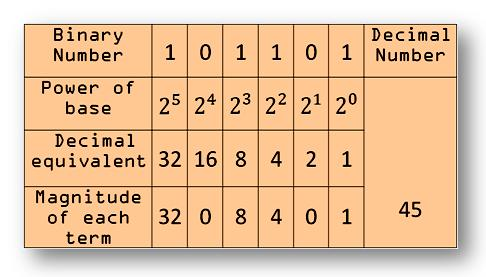
\includegraphics[width=0.6\textwidth]{images/binary.jpg}
    \caption{A table illustrating how to convert the binary number 101101 into its decimal equivalent, 45 \cite{binary}}\label{fig:BINARY}
\end{figure}
\subsubsection{How is a bit physically stored?}
Use figure here
\subsubsection{Gates - Manipulating bits}
\begin{figure}[H]
    \centering
    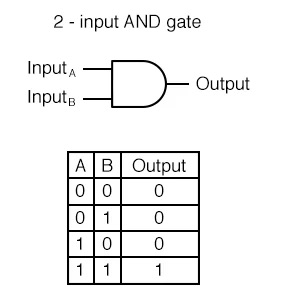
\includegraphics[width=0.4\textwidth]{images/andgate.jpeg}
    \caption{The circuit symbol for an AND gate, along with a true table of all possible outputs for two inputs, A and B. \cite{andgate}}\label{fig:ANDGATE}
\end{figure}
\subsubsection{Computation - Many gates}
\begin{figure}[H]
    \centering
    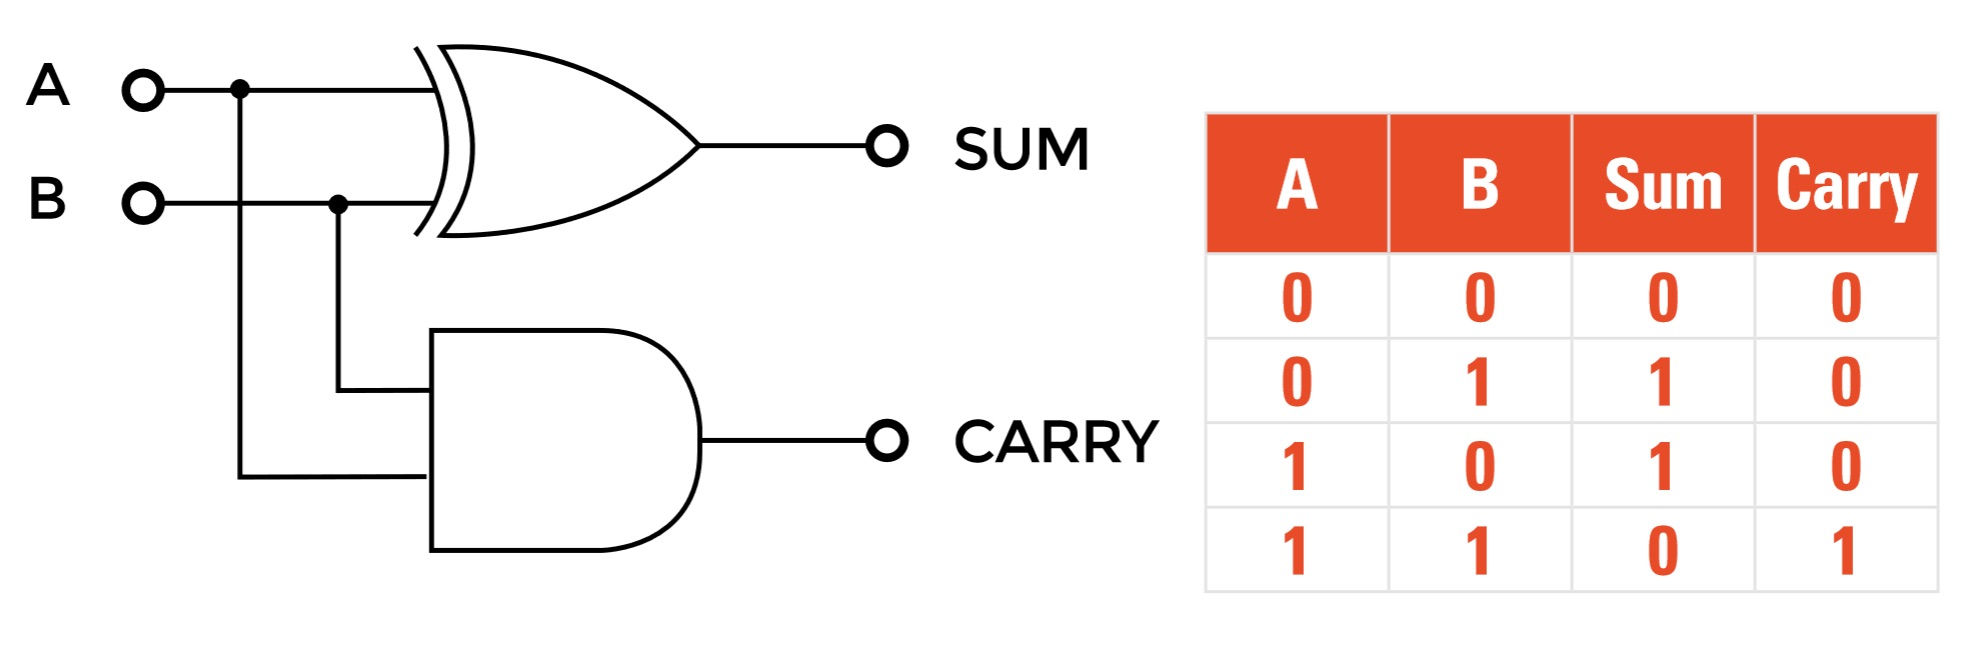
\includegraphics[width=0.7\textwidth]{images/adder.jpeg}
    \caption{A logic diagram of a binary half adder, including truth table output for all possible input combinations. \cite{adder}}\label{fig:ADDER}
\end{figure}

\subsection{Relevant Quantum Physics}

Quantum computing's advantages are a direct result of the quantum mechanical properties such as superposition and entanglement that distinguish it from classical computers. 
These two properties along with quantum teleportation and the Bell inequality will be discussed.
Finally decoherence times of quantum states will be introduced as a means of demonstrating the difficulty with scailability in quantum computing. 



\subsubsection{Superposition}
Superposition is a quantum mechanical phenomenon where an object may exist in multiple states at once. 
For example an electron may be said to be in two places at once - or more accurately its probability function covers multiple areas in space. \cite{noauthor_whatCal_nodate}

Superposition can be observed in the polarisation of light. 
Light can be horizontally, vertically and circularly polarized and much of the light around us is a superposition of the three.
However when light interacts with surfaces their properties can change such as light reflecting off a pond being horizontally polarized. 
Using a linear polariser one can control the direction of polarisation of the light passing through it.
Constructing two polarisers at right angles (vertical and horizontal respectively) one would expect only vertical polarised light to emitted from the first and then no light to be emitted from the second polariser. 
This is what is experimentally observed - however if a third polariser is placed between the horizontal and vertical polarisers orientated at 45$^\circ$ (as in figure \ref{fig:polarisers}) from both then light will now be transmitted through the final horizontal polariser (at 50$\%$ intensity). \cite{noauthor_whatCal_nodate}
This also emphasises this highly probabilistic behavior of QM where after exciting the second polariser the light is again a superposition of all the states that produce the diagonal polarisation. {\bf make this sentence clearer}
!!! make the link to superposition clearer here!!!

\begin{figure}[H]
  \centering
  \begin{subfigure}[b]{0.44\linewidth}
    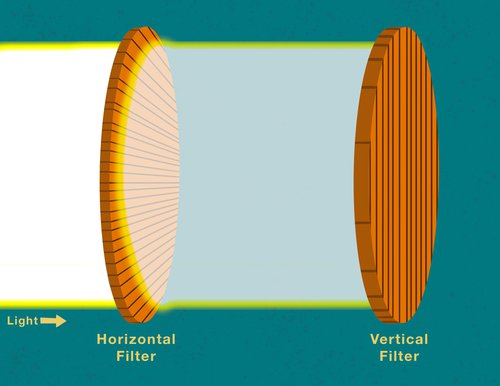
\includegraphics[width=\linewidth]{images/2 polariser.jpg}
    \caption{Unpolarised light passing through a horizontal and then failing to pass through a vertical polarising filter. }\label{fig:2 polarise}
  \end{subfigure}
  \begin{subfigure}[b]{0.44\linewidth}
    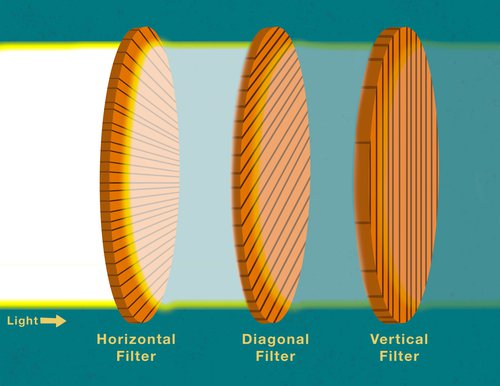
\includegraphics[width=\linewidth]{images/3 polariser.jpg}
    \caption{Unpolarised light passing through three successive polarising filters. A horizontal and vertical filter and a linear polariser orientated 45$^\circ$ between both. }\label{fig:3 polarise}
  \end{subfigure}
  \caption{Unpolarised light passing through linear polarising filters in two set ups. \cite{noauthor_whatCal_nodate}}
  \label{fig:polarisers}
\end{figure}

It is this superposition of states which allows a single qubit to trial multiple values at once. \cite{sonialopezbravo_understanding_nodate}

\subsubsection{Entanglement}
Entanglement is a uniquely quantum mechanical phenomenon where the measurement of one particle's state will effect the state of another particle.
I.e. for interacting states A and B their combined wavefunction cannot be expressed as the product of the individual wavefunctions of A and B if states A and B are entangled. \cite{bransden_quantum_2000}
\vspace{1em}
For example the LHS of equation \ref{eqn:superqubit} is not an entangled system (simply a superposition of states) as it can be expressed as the tensor product of both wavefunctions.

\begin{equation}\label{eqn:superqubit}
    |0\rangle_\phi|0\rangle_\psi + |0\rangle_\phi|1\rangle_\psi + |1\rangle_\phi|0\rangle_\psi +
    |1\rangle_\phi|1\rangle_\psi = |\phi\rangle \otimes |\psi\rangle
\end{equation}

However the system in equation \ref{eqn:entqubit} is entangled as the total system cannot be expressed as a product of the two single systems. 
\begin{equation}\label{eqn:entqubit}
    \frac{|0\rangle_\phi|0\rangle_\psi + 
    |1\rangle_\phi|1\rangle_\psi}{\sqrt{2}}
\end{equation}

The state in equation \ref{eqn:entqubit} is particularly interesting and is known as the bell state (the $\sqrt{2}$ is a normalising factor).
It is 2-Qubit entangled state which is used frequently in quantum computing and can be achieved by applying a `Hadamard' and `cNOT' quantum gates to two qubits. \cite{mermin_quantum_2007} 
{\bf check if mathew talks about quatum gates yet}
Measuring only one of the qubits in this state would also reveal the state of the other qubit. 
If a $|0\rangle$ is measured from one qubit then the other qubit must also be $|0\rangle$ while if a $|1\rangle$ is measured then the other qubit must also be in a $|1\rangle$ state. 
The probability of measuring $|0\rangle$ is 50$\%$ and similarly for measuring $|1\rangle$. 

\vspace{1em}

Although progress has been made in studying quantum entanglement, there is no complete theory to explain it. 
It does play an integral role in quantum computing however and deeper investigation of it and how to manipulate this property is likely to lead to further applications. \cite{nielsen_quantum_2010}

\vspace{1em}

One exciting application is quantum teleportation

\subsubsection{quantum teleportation}

\subsubsection{Bell State}

\subsubsection{decoherence of states}

\subsubsection{no cloning theorem}




\subsection{The DiVincenzo Criteria -- to be polished}
The DiVincenzo criteria is a set of objectives that must be met for the physical realisation of a quantum computer. 
It sets out five basic principles which must met to build a functional quantum computer and two more principles for quantum information networks. \cite{bergou_quantum_2021}
This report focuses on the implementation of a single quantum computer and therefore focused on the first five principles.
The principles are:
\begin{enumerate}
    \item Scalability with well defined qubits
    \item The ability to initialise the system in a well defined, determinate state
    \item The ability to read out qubit state with high accuracy
    \item A set of universal quantum gates
    \item Long relevant decoherence times
    \newcounter{enumTemp}
    \setcounter{enumTemp}{\theenumi}
\end{enumerate}
The two principles for the implementation of quantum information networks are:
\begin{enumerate}
    \setcounter{enumi}{\theenumTemp}
    \item The ability to convert between `stationery' and `flying' qubits
    \item The ability to transmit flying qubits between specified locations
\end{enumerate}

There are various physical approaches for quantum computing that satisfy some of the DiVincenzo criteria, however no current approach has successfully satisfied all five.
\vspace{1em}

The first objective to implement well defined qubits which are saliable. An example of a well defined qubit is superposition of vertical and horizontal polarisation of a photons, or the spin up and spin down of electrons. 
There are many methods of creating well defined qubits, however scalability and producing multiple which remain in a superposition state is challenging.
IBM claimed in 2021 to have created the worlds largest quantum processor, the 127 qubit Eagle. \cite{authorfullname_ibm_nodate}
\vspace{1em}

The second objective is to initialise the qubits into a well defined determinate state i.e. initialise the qubit register so all are in the 0 state $\vert 0\rangle \vert 0\rangle$...$\vert 0 \rangle$. \cite{lapierre_divincenzo_2021}
\vspace{1em}

The third objective is to read out qubit state $\vert 0\rangle$ or $\vert 1 \rangle$ with high accuracy. 
This is a challenge with photons as a method for detecting individual photons with no dark count (false positives) does not exist yet.
\vspace{1em}

The fourth objective is to implement a universal set of gates, all operations can be preformed using two quantum gates.
One is gate which flips the state of a single qubit. The other is a CNOT gate which acts on two qubits and flips the state of one qubit only if the 'control' qubit is in state $\vert 1 \rangle$. \cite{lapierre_divincenzo_2021} 
\vspace{1em}

The final objective is for long `relevant' decoherence times, this requires the qubit to stay in a superposition quantum state for longer than the duration of gate operations before the state collapses. 
